\chapter{The Booster Neutrino Beam}\label{ch:beam}

The MicroBooNE detector is stationed at Fermi National Accelerator Laboratory (FNAL) where it receives neutrinos from both the Booster Neutrino Beam (BNB) and Neutrinos from the Main Injector (NuMI) beams. MicroBooNE is on-axis for the BNB and off-axis by 135 mrad for NuMI. For the purpose of this analysis, only data from the BNB was used. This chapter will discuss how neutrinos are created using the BNB. How these neutrinos are produced as well as their flux through the MicroBooNE detector is necessary for any analysis because of the systematic uncertainties the beam introduces to a measurement.

\section{Creating the Booster Neutrino Beam}
The BNB is a very pure $\nu_{\mu}$ beam, with only 0.6\% contamination from $\nu_{e}s$. The energy also peaks around 700 MeV which is desired based on the probability of oscillation equation which depends on the the value of $L/E$, where $L$ is the distance of the detector from the neutrino beam and $E$ is the energy of the neutrino beam. $L/E$ was chosen to increase the probability of seeing neutrino oscillations in the MiniBooNE Low Energy Excess (LEE) range based on the probability of oscillation equation, which is $ P_{\nu_{\mu}\rightarrow \nu_{e}}\left(L,E\right) = \sin^2 2\theta \sin^2 \left(1.27\Delta m^2 \frac{L}{E_{\nu}}\right)$. The BNB collides 8.9 GeV/c momentum protons from the FNAL booster synchrotron into a beryllium target which produces a high flux of neutrinos. The protons originate from $H^2$ gas molecules that are turned into $H^-$ ions by a Cockroft-Walton generator shown in figure \ref{fig:generator}. The $H^-$ initially are accelerated to 1MeV kinetic energy and are then passed to a linear accelerator using alternating electromagnetic fields to increase their energy to ~400MeV. The ions are stripped of electrons by passing them through a carbon foil. The protons are bunched into beam spills which contain ~$4*10^12$ protons in a 1.6 $\micro s$ time window per spill. It's at this point that the protons are directed towards the beryllium target. The amount of protons directed towards the target (POT) is measured by two toroids upstream of the target with an error of ~2$\%$. Beam intensity, timing, width, position, and direction are monitored by beam position monitors, multi-wire chamber and resistive monitors. 
The beryllium target is 71.1 cm long, 1.7 proton interaction lengths, and is 0.51 cm in radius. The target is located inside a larger focusing electromagnet called the horn. THe horn is an aluminum alloy pulsed toroidal electromagnet. The pulsed current peaks at 170 kA with a time-width of 143 $\micro s$ which coincides with the protons arriving on the target. The current flows from the inner conductor to the outer conductor with a maximum magnetic field of 1.5 Tesla. The magnetic field focuses the charged secondary particles produced by the p-Be interactions. The direction of current can be switched to changed to polarity of the secondary particles being focused creating a beam of either primarily neutrinos, with positively charged secondary particles, or antineutrinos. 

Further down the beamline is a concrete collimator which absorbs particles not necessary to the neutrino flux. The collimator is 214 cm long and ~ 30 cm in radius. After the collimator comes a 45 meter long, 1 meter raduis, air-filled cylindrical decay region which then ends in a beam-stop made of steam and concrete. The beam-stop contains an array of gas proportional counters to detect muons. \text{red}{\textbf{add beam diagram here}}     





\begin{figure}[htp!]
\centering
	\begin{subfigure}[b]{.4\textwidth}
	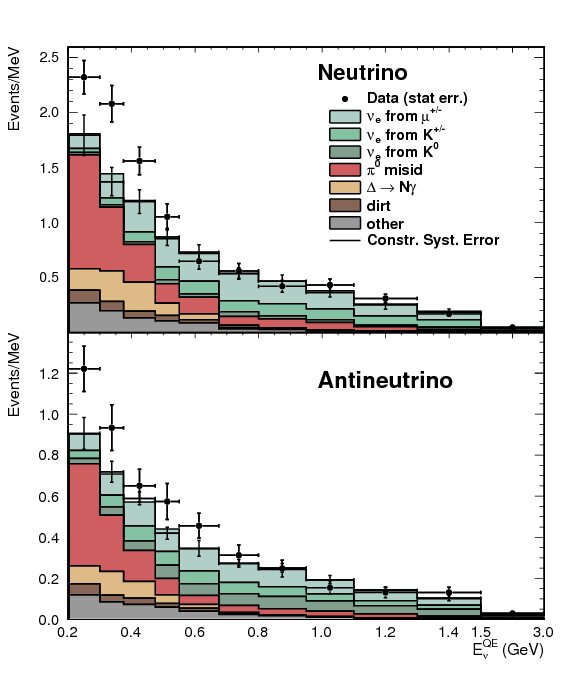
\includegraphics[width=\textwidth]{figs/lee.png}
	\caption{Low Energy excess seen in MiniBooNE}
	\label{fig:lee}
	\end{subfigure}
	\quad
	\begin{subfigure}[b]{.4\textwidth}
	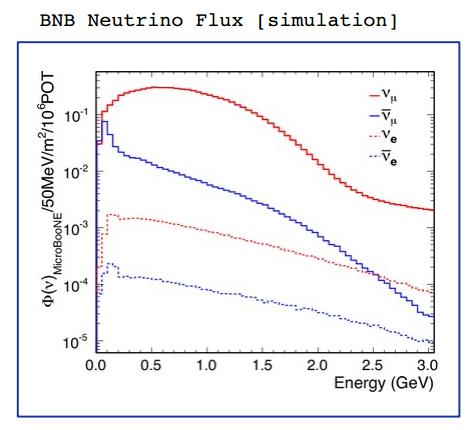
\includegraphics[width=\textwidth]{figs/bnbflux.png}
	\caption{Energy spectrum of the Booster Neutrino Beam at Fermi National Laboratories}
	\label{fig:bnbflux}
	\end{subfigure}
	\quad
\label{fig:figures}
\caption{\ref{fig:bnbflux} Flux of BNB at FNAL.}
\end{figure}
